% !TeX program = lualatex
\documentclass[10pt,conference,a4paper]{IEEEtran}
\usepackage[utf8]{inputenc}
\usepackage[T1]{fontenc}
\usepackage[rm={oldstyle=false}]{cfr-lm}
\usepackage[australian,american]{babel}

\usepackage[backend=biber,style=ieee,bibencoding=utf8,sorting=none,doi=false,isbn=false,url=false,date=short]{biblatex}
\usepackage{amssymb}
\usepackage[cmex10]{amsmath}
\usepackage{csquotes}
\usepackage{cleveref}
\usepackage[nolist]{acronym}
\usepackage{float}
\usepackage{todonotes}
\usepackage{pgfplots}
\usepackage{pgf}
\usepackage[binary-units]{siunitx}
\usepackage{pgfplotstable}
\usepackage{booktabs}
\usepackage{multirow}
\usepackage{lipsum}
\usepackage[hidelinks]{hyperref}
\usepackage{xspace}
\usepackage[caption=false]{subfig}

\usetikzlibrary{patterns}

\usepgfplotslibrary{external, groupplots, units}
\tikzexternalize
\tikzsetexternalprefix{generated-figures/}

\sisetup{
	round-mode          = places,
	round-precision     = 2,
}
\DeclareSIUnit\mbps{MB/s}
\DeclareSIUnit\gbps{Gb/s}



\pgfplotscreateplotcyclelist{my colors}{%
solid, color=black\\%
densely dotted, color=blue\\%
densely dashed, color=red\\%
}
\makeatother

%% Environment for comments: Set the boolean to false to produce a comment-free version.
\newboolean{showcomments}
\setboolean{showcomments}{true}
\ifthenelse{\boolean{showcomments}}
{ \newcommand{\mynote}[3]{
		\fbox{\bfseries\sffamily\scriptsize#1}
		{\small$\blacktriangleright$\textsf{\textit{\color{#3}{#2}}}$\blacktriangleleft$}}}
{ \newcommand{\mynote}[3]{}}
% One command per author:
\newcommand{\jt}[1]{\mynote{Jocelyn}{#1}{blue}}
\newcommand{\hm}[1]{\mynote{Hugues}{#1}{orange}}

\newcommand{\epto}{\textsc{EpTO}\xspace}
\newcommand{\jgroups}{\textsc{JGroups}\xspace}
\newcommand{\eptotester}{\textsc{EpTOTester}\xspace}

\newif\ifjmcs
% Change false to true to have the JMCS cover page
\jmcstrue

\pgfplotsset{
	% compat=1.14,
	tick label style={font=\small},
	label style={font=\small},
	legend style={font=\small},
	/pgfplots/short line legend/.style={
		legend image code/.code={
			\draw[mark repeat=2,mark phase=2,##1]
			plot coordinates {
				(0cm,0cm)
				(0.2cm,0cm)
				(0.4cm,0cm)
			};%
		}
	},
	/pgfplots/xtick pos=left,
}

\def\ieeetitle{EpTOTester}
\def\ieeeauthor{X,X,X}

\def\thesistitle{EpTOTester}
\def\thesissubtitle{Implementation of Large-Scale Epidemic Total Order Algorithms
}
\def\thesisauthor{Jocelyn Thode}


\author{\IEEEauthorblockN{\ieeeauthor}
	\IEEEauthorblockA{University of Fribourg, Switzerland\\
		\href{mailto:first.last@unifr.ch}{first.last@unifr.ch}}
}
\title{\ieeetitle}

\addbibresource{references.bib}
\renewcommand*{\bibfont}{\small}

\hypersetup{
	pdftitle=\thesistitle,
	pdfauthor=\thesisauthor
}

% \noautocite{*}


\begin{document}
	
\ifjmcs
\begin{titlepage}
	\begin{otherlanguage}{australian}
		\begin{center}
			\begin{figure}[t]
				\center{
\includegraphics[scale=0.2]{logos/MSc_quer.png}}
				\vspace{0.4in}
			\end{figure}
			
			{\bfseries\Huge \thesistitle \par
				\Large \vspace{0.1in} \thesissubtitle \par}
			
			\vspace{0.3in}
			\LARGE{\textbf{Master Thesis} \\}
			\vspace{0.4in}
			
			{\Large \thesisauthor}
			
			\vspace{0.3in}
			{\Large Université de Fribourg \par}
			\vfill
			{\Large \today \par}
			
			\vspace{0.9in}
			
			% === Logos ==============================================
			\begin{figure}[htp]
				\centering
				\subfloat{
\includegraphics[scale=0.60]{logos/UNI_Bern.pdf}}\hfill
				\subfloat{
\includegraphics[scale=0.54]{logos/UNI_Neuchatel.pdf}}\hfill
				\subfloat{
\includegraphics[scale=0.81]{logos/UNI_Fribourg.pdf}}
			\end{figure}
			% === // Logos ==========thun=================================
			
		\end{center}
	\end{otherlanguage}
\end{titlepage}

\pagebreak
\fi

%	\maketitle
	
\begin{abstract}
\epto is one of the recently introduced total order algorithms for large-scale distributed systems and claims to provide total order and scalability at the same time. In this paper, we verify this claim by implementing EpTO \autocite{matos2015epto} and evaluate its reliability in real-world conditions by comparing it to a deterministic total order algorithm named \jgroups. We first compare them in a perfect environment assessing the scalability in terms of events throughput and peer numbers. We then compare them using a synthetic churn trace and a real one using the same metrics. Our results shows \epto is performing has expected, although further testing on a bigger cluster is required to evaluate how it performs when \jgroups no longer does.
\end{abstract}
\section{Introduction}
\jt{If we present it as a framework we need to find a new name}

Creating an algorithm providing scalability, integrity and validity, along with a total ordering of the events through all peers in a distributed network has been one the hot topics in distributed computing research for many years. There are many algorithms for disseminating and ordering events in a distributed network. There are deterministic algorithms, which guarantee total order, agreement or other strong properties. Unfortunately, these types of algorithms are not scalable enough to be used in large-scale distributed systems \autocites[]{defago2004total}[]{lamport1978time}.
\par
The problem with existing deterministic total ordering protocols is that they need some sort of agreement between all peers in the network. This causes a massive amount of network traffic and overhead on the system.
Moreover, an agreement feature for an asynchronous system requires to
explicitly maintain a group and have access to a failure detector \autocites[]{chandra1996weakest}[]{chandra1996unreliable}. Due to faults and churn in large-scale distributed systems, the failure detector turns into a bottleneck for the structure and thus limits the algorithm's scalability.
\par
As an alternative to deterministic algorithms, there are probabilistic algorithms, focusing on scalability and resiliency against failures using a probabilistic dissemination approach  \autocite{birman1999bimodal,carvalho2007emergent,demers1987epidemic,eugster2003lightweight,felber2002probabilistic,hayden1996probabilistic,kim2004gossip,Koldehofe02simplegossiping}. These algorithms guarantee the dissemination of events in the system with high probability. This way, there is no need for failure detectors and redundant traffic, making these algorithms highly scalable. As these algorithms focus on reliability of dissemination, they often have to ignore other properties such as total ordering. 

One of the recently designed algorithms in the field is \epto \autocite{matos2015epto}. \epto is an algorithm that claims to solve these seemingly irreconcilableŝ
differences. Furthermore, \epto is designed to work without a global clock, removing the need to synchronize clocks precisely on every peer and thus is well-suited for these kind of systems.
\par
By using a probabilistic dissemination together with deterministic ordering, \epto provides total order along with scalability, validity and integrity. \epto consists of two distinct components. \epto's dissemination component guarantees that all peers will receive an event with arbitrarily high probability. Once peers have received all events, \epto's ordering component orders them using the events timestamp, and in case of a tie use the broadcaster ID of the events.
\par
To model the first component, \epto is using a \textit{balls-and-bins} approach \autocite{Koldehofe02simplegossiping}. The \textit{balls-and-bins} problem is a basic probabilistic problem: consider \textit{n} balls and \textit{m} bins where we consequently throw balls into a bin uniformly at random and independently from other balls. In this scenario, one of the natural questions that comes to mind is: what is the minimum number of balls that should be thrown, so that every bin has at least one ball with high probability?
\begin{figure}
	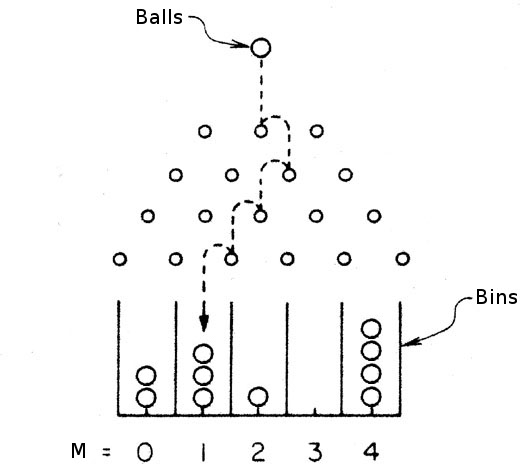
\includegraphics[width=\linewidth]{figures/BnB.jpeg}
	\caption[Caption]{Balls-and-Bins\footnotemark}
	\label{fig:balls-and-bins}
\end{figure}
\footnotetext{Figure inspired from \autocite{bnb}}
\par
Using the balls-and-bins approach we model processes as bins and events as balls and calculate how many balls need to be \textit{thrown} such that every bin contains at least one ball with arbitrarily high probability. With this approach the number of messages transmitted per process per round is logarithmic in the number of processes, therefore the number of messages sent in the system is low and uniform over all processes. Thanks to these approaches, \epto is highly resilient with  imperfect networks and highly scalable as the networks grow, while always providing total order.
\subsection{Contributions}
Until now, the creators of \epto have only tested this algorithm in a simulated environment. In this work, we implement \epto in pure Kotlin\footnote{\href{https://kotlinlang.org/}{https://kotlinlang.org/}} and introduce a benchmarking framework called \eptotester to show that \epto is suitable for real-world large-scale distributed systems. We compare \epto to the deterministic total order algorithm provided by \jgroups \autocite{jgroups} in both stable and unstable environments. \epto uses a PSS CYCLON \autocite{Voulgaris2005} to obtain a random view. Peers use a tracker that keeps track of dead and alive peers when they first join the network. These benchmarks can easily be launched and scaled on a cluster using Docker and Docker Swarm. Furthermore, we can inject synthetic or real churn using the Failure Trace Archive databases\footnote{\href{http://fta.scem.uws.edu.au/}{http://fta.scem.uws.edu.au/}} in the system. \eptotester is open-sourced on Github\footnote{\href{https://github.com/jocelynthode/EpTOTester}{https://github.com/jocelynthode/EpTOTester}}. Finally we want to emphasize that few works evaluate such protocols in a really large scale \autocites[]{Chandra2007}[]{Maia2011}.
\par
The next sections present our benchmarking solution and the results obtained. Section \ref{sec:background} exposes the background of \eptotester and presents the different kind of ordering. Section \ref{sec:definitions} defines the terms used in the paper. Section \ref{sec:epto} presents \epto and the architecture of our implementation. Section \ref{sec:evaluation} shows and explains the results obtained as well as the limitations our project faced. We then present possible future work in Section \ref{sec:future-work}. We finally conclude in Section \ref{sec:conclusion}.

\section{Ordering Algorithms}
\label{sec:ordering}
Distributed systems and centralized systems alike, need to preserve the temporal order of events produced by concurrent processes in the system. When there are separated processes that can only communicate through messages, you cannot easily order these messages.
Therefore we need ordering algorithms to overcome this problem.
\par
We have two types of ordering algorithms \autocite{lamport1978time}: the partial order algorithms and the total order algorithms.
\subsection{Partial Order Algorithms}
Assuming S is partially ordered under $\leq$, then the following statements hold for all a, b and c in S:
\begin{itemize}
	\item Reflexivity: $a \leq a$ for all $a \in S$.
	\item Antisymmetry: $a \leq b$ and $b \leq a$ implies $a=b$ .
	\item Transitivity: $a \leq b$  and $b \leq c$  implies $a \leq c$.
\end{itemize}

\subsection{Total Order Algorithms}
A totally ordered set of events is a partially ordered set which satisfies one additional property:
\begin{itemize}
	\item Totality (trichotomy law): For any $a, b \in S$, either $a \leq b$  or $b \leq a$.
\end{itemize}
\par
In other words, total order is an ordering that defines the exact order of every event in the system. On the other hand, partial ordering only defines the order between certain key events that depend on each other. Partial order can be useful since it is less costly to implement. However, in some cases the order of all events is important. For example, imagine we have multiple databases around the world. We want them to appear as if it is only one database. To achieve this, every operation done a particular database would have to be replicated on all the others, we would then have to make sure that every operation is executed in the same order on every database to end up in the same state. \hm{It would be enlightening to be more precise here and add a large-scale distributed application for which total order is important.}\jt{I came up with a possible total order application. However I am not sure if it is the best use case. Maybe Miguel has a better idea.}

\section{Definitions}
A process or peer is defined as an actor in our system running the application that needs total order. Each process will communicate with other processes in the distributed system, exchange events, and order them together.
\par
An event is defined as data sent at a given time by a peer. For example, we could imagine a system where each process publishes some data to other peers. The moment where we publish data combined with the data is called an event.
\par
A ball is a set of events bundled together and sent as one package. We use balls in \epto to reduce network traffic and make it scalable in terms of processes and events.

We define \epto scaling well as it was defined in  \autocite{matos2015epto}:  ``The number
of messages transmitted per process per round is logarithmic
in the number of processes, ...''. The number of rounds needed to deliver an event stays low as well.
\par
Since \epto uses a probabilistic agreement instead of a deterministic agreement, there might be a situation where a peer does not receive an event (with a very low arbitrary probability). In this instance there will be a hole in the sequence of delivered events but even in this case, the order of the delivered events will be protected by \epto's deterministic ordering algorithm, thus the total order property is preserved.
\par
We write the cluster parameters as $(p,e)$, where $p$ designates the total number of peers and $e$ designates the global event throughput. We tested \epto and \jgroups with three different cluster parameters:
\begin{description}[\IEEEsetlabelwidth{$(100,100)$:}]
	\item[\textbf{$(100,100)$}:] 50 peers with a global event throughput of 50 events per seconds.
	\item[\textbf{$(100,100)$}:] 50 peers with a global event throughput of 100 events per seconds.
	\item[\textbf{$(100,100)$}:] 100 peers with a global event throughput of 50 events per seconds. This parameter was also used for all synthetic churns.
\end{description}
\par

\section{EpToTester}
\label{sec:epto}
\eptotester is a framework using Docker and Docker Swarm. It is designed to ease the deployment of large scale distributed systems and in this particular case \jgroups and \epto. We use \eptotester to assess the claims made in \autocite{matos2015epto}. Although the implementation of \epto is written with benchmarking in mind, the code can be adapted for real applications with only minimal changes to the sources. We  use \eptotester instead of other solutions such as SPlay, which only supports LUA, as we need to test existing protocols written in different programming languages.
\subsection{Deployment}
\begin{figure}[htp]
	\centering
	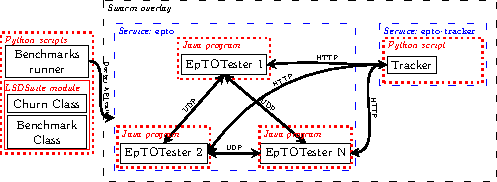
\includegraphics[width=\linewidth]{figures/complete-architecture.pdf}
	\vspace{-2mm} 
	\caption[Caption]{\epto using the \eptotester\mm{this needs to be explained in more detail in the text in particular the concept of different services, the benchmark, etc. the churn modules are also missing} framework\footnotemark}
	\vspace{-2mm} 
	\label{fig:complete-architecture}
\end{figure}
\footnotetext{This figure is partially inspired from a figure in \autocite{vaucher2016erasure}}
To deploy a protocol in our framework we need two different Docker Swarm services: one containing the tracker and one containing all replicas. Both of these services use the same network overlay to communicate. This is achieved using Docker and especially the new Docker Swarm introduced in Docker 1.12. This lets us have a unified way of deploying our benchmarks locally or remotely on vastly different clusters with minimal modifications. Every benchmark is started through a Python script available on the master node. This script handles everything from starting benchmarks, scaling the cluster during a churn and collecting results through the framework Python classes. Application, churn and cluster  parameters are customizable through YAML configuration files. Tracker and replica communication is up to the user. For example, \epto uses HTTP, while \jgroups uses TCP directly. Tracker implementation is also left to the user, although a REST Tracker implemented in Python is provided by default. The user can also opt to not use a tracker at all.
Gradle\footnote{\href{https://gradle.org/}{https://gradle.org/}} is used to automate the project building. Finally, a script is provided to push the images to a repository accessible to the remote cluster and to push the benchmarking framework on the master node. \jgroups uses the same deployment method. Our framework applied to \epto can be seen in \autoref{fig:complete-architecture}.
\subsection{Fault Injection}
Our framework supports the ability to inject synthetic and real traces thanks to the work done in \autocite{vaucher2016erasure}. The synthetic churn provided by it was improved to support adding and removing nodes at the same time\mm{point out that when this is simultaneous it applies to different sets of nodes.}.

Synthetic churn follows strict periods. Every period of time, it modifies the cluster size according to the instructions until there are no more steps. These instructions can either: do nothing, increase the cluster size, reduce the cluster size or both at the same time.

Real traces are based on FTA traces as stated earlier. Every time we query the database, we obtain every cluster change that happened since the last query according to the trace and the time elapsed between both queries. Thus, the smaller the period, the more accurate it is regarding to the real trace.
\subsection{Extensions}
\eptotester is a general framework and should satisfy most decentralized applications needs with almost no tweaking. However, some protocols are centralized. This is the case for \jgroups. \jgroups relies on MULTICAST and has a coordinator that orders every events sent. \eptotester is written such that the main Benchmark and Churn modules are extensible to suit any need, thanks to class inheritance. In our experiments we wrote an extension of the Churn module, so that it can deal with the coordinator, killing it only when we want to. This provides us with fine-grained control over the benchmarks. 

\eptotester supports the use of a tracker as a separate service. If the application using the framework needs a tracker it only has to provide the docker image name for the tracker in the application configuration YAML file for the tracker to be created alongside the application service.
\subsection{Protocols Implementation}
We implement the network layer using UDP and our own PSS CYCLON operating on its own port to obtain a random view of peers. To obtain an initial random view, we contact an independent tracker implemented as a simple Python web server that keeps track of dead and alive nodes in the system using GET requests. We want to emphasize that the tracker is not required. In practice it works well, but using a DHT is certainly a possibility.

We implement the payload as randomly generated UUIDs. We compare \epto to the deterministic total order algorithm SEQUENCER provided by \jgroups. We use \jgroups 3.6.11. When implementing \jgroups we use TCPGOSSIP \autocite{tcpgossip} provided by the \jgroups library as a tracker instead of the traditional MULTICAST option to coordinate peers, as Docker services do not yet support MULTICAST. This is not a problem as in a real WAN \jgroups could not rely on MULTICAST\mm{reference the jgroups page where they mention this}.

The \epto simulation and theory is assuming we can have balls of infinite size which of course is not possible in practice.
We must therefore limit the ball size to a practical number. We use balls with a maximum size of \SI{1432}{\byte}. We choose this number as the default MTU on Ethernet is \SI{1500}{\byte}. We then subtract the bytes required for the IPv4 and UDP headers.

When benchmarking \jgroups we have to send a SIGSTOP to the containers instead of killing them, as otherwise the kernel closes the TCP connection to the TCPGOSSIP nicely, making it appear as a regular leave instead of a failure. SIGSTOP lets us simulate a harsh connection drop.


\section{Evaluation}
\label{sec:evaluation}
\jt{specify somewhere the problems encountered with JGroups}
\pgfplotstableread[col sep=comma]{csv-data/average-bytes-sent-recv.csv}\tableaverage
\pgfplotstableread[col sep=comma]{csv-data/plot-global-time-cdf.csv}\tableglobaltime
\pgfplotstableread[col sep=comma]{csv-data/plot-local-deltas-cdf.csv}\tablelocaldeltas
\pgfplotstableread[col sep=comma]{csv-data/plot-local-time-cdf.csv}\tablelocaltime
In this section we present our results. In the following benchmarks \epto uses a constant $c$ to set the probability of a hole appearing. We set $c = 4$ in all our benchmarks so as to not experience any holes as \jgroups does not produce holes under normal conditions. We use a $\delta$ period of \SI{100}{\milli\second} for tests with no churn or synthethic churn and \SI{250}{\milli\second} for tests following a real trace.
\par 
We used specific settings recommended by \jgroups for a big cluster.
\par
Every \jgroups test run with churn is run once killing the coordinator and once not killing it. We use the following nomenclature to differentiate both tests:
\begin{description}[\IEEEsetlabelwidth{\jgroups-nocoord: }]
	\item[\textbf{\jgroups-coord}:] The coordinator is killed once
	\item[\textbf{\jgroups-nocoord}:] The coordinator is purposely kept alive
\end{description}
\par
\textbf{Testbed.} Our cluster is comprised of... \jt{Ask Valerio+Seb and speak about the different software needed}
\par
\textbf{Experiment parameters.} Every benchmark except the one following a real trace are run 10 times, each during \SI{20}{\minute}. When there is synthetic churn, the churn starts \SI{30}{\second} after the benchmark and run for \SI{17}{\minute}. The benchmarks following a real trace are run 5 times. The trace is speed-up 2x, which means we follow \SI{2}{\hour} in \SI{1}{\hour}. Every benchmark run with churn is run with the $(100,50)$ parameters.
\subsection{Bandwidth}
\begin{figure}[hpt]
	\centering
	\begin{tikzpicture}
\usetikzlibrary{plotmarks}
\pgfplotsset{
	height=4cm,
	width=\linewidth / 2.6,
	every axis plot post/.append style={
		solid,
		very thin,
		mark=none
	},
	/pgfplots/area cycle list/.style={/pgfplots/cycle list={%
			{black,fill=black,mark=none},%
			{black,fill=white!25!black,mark=none},%
			{black,fill=white!50!black,mark=none},%
			{black,fill=white!75!black,mark=none},%
			{black,fill=white,mark=none},%
		}
	},
}
\begin{groupplot}[
ymajorgrids,
group style={
	group size=3 by 2,
	vertical sep=8mm,
	horizontal sep=4mm,
	xlabels at=edge bottom,
	ylabels at=edge left,
	yticklabels at=edge left,
},
stack plots=y,area style, enlarge x limits=false, 
ymin=0,
xmin=0,
ymax=4.5,
ytick={0,1,2,3,4},
yticklabels={0,1,2,3,4},
ylabel={Bandwidth $\left[\SI{}{\mbps}\right]$},
xlabel={Time $\left[\si{\minute}\right]$},
legend columns=5,
legend cell align=left,
legend style={at={(1.8,1.5)},anchor=north, font=\small, draw=none, fill=none},]
\nextgroupplot[ymax=4,ytick={0,1,2,3,4},
yticklabels={0,1,2,3,4},]
\addplot table[x=time,y=EpTO-50-1sec-0.000000, col sep=comma]{\tableaverage} \closedcycle;
\addplot table[x=time,y=EpTO-50-1sec-0.250000, col sep=comma]{\tableaverage} \closedcycle;
\addplot table[x=time,y=EpTO-50-1sec-0.500000, col sep=comma]{\tableaverage} \closedcycle;
\addplot table[x=time,y=EpTO-50-1sec-0.750000, col sep=comma]{\tableaverage} \closedcycle;
\addplot table[x=time,y=EpTO-50-1sec-1.000000, col sep=comma]{\tableaverage} \closedcycle;
\legend{0, 0.25, 0.5, 0.75, 1}
%
\nextgroupplot[ymax=4,ytick={0,1,2,3,4},]
\addplot table[x=time,y=EpTO-50-2sec-0.000000, col sep=comma]{\tableaverage} \closedcycle;
\addplot table[x=time,y=EpTO-50-2sec-0.250000, col sep=comma]{\tableaverage} \closedcycle;
\addplot table[x=time,y=EpTO-50-2sec-0.500000, col sep=comma]{\tableaverage} \closedcycle;
\addplot table[x=time,y=EpTO-50-2sec-0.750000, col sep=comma]{\tableaverage} \closedcycle;
\addplot table[x=time,y=EpTO-50-2sec-1.000000, col sep=comma]{\tableaverage} \closedcycle;
%
\nextgroupplot[ymax=4,ytick={0,1,2,3,4},]
\addplot table[x=time,y=EpTO-100-1sec-0.000000, col sep=comma]{\tableaverage} \closedcycle;
\addplot table[x=time,y=EpTO-100-1sec-0.250000, col sep=comma]{\tableaverage} \closedcycle;
\addplot table[x=time,y=EpTO-100-1sec-0.500000, col sep=comma]{\tableaverage} \closedcycle;
\addplot table[x=time,y=EpTO-100-1sec-0.750000, col sep=comma]{\tableaverage} \closedcycle;
\addplot table[x=time,y=EpTO-100-1sec-1.000000, col sep=comma]{\tableaverage} \closedcycle;
%
\nextgroupplot[ymax=1.5,ytick={0,0.5,1,1.5},yticklabels={0,0.5,1,1.5},]
\addplot table[x=time,y=JGroups-50-1sec-0.000000, col sep=comma]{\tableaverage} \closedcycle;
\addplot table[x=time,y=JGroups-50-1sec-0.250000, col sep=comma]{\tableaverage} \closedcycle;
\addplot table[x=time,y=JGroups-50-1sec-0.500000, col sep=comma]{\tableaverage} \closedcycle;
\addplot table[x=time,y=JGroups-50-1sec-0.750000, col sep=comma]{\tableaverage} \closedcycle;
\addplot table[x=time,y=JGroups-50-1sec-1.000000, col sep=comma]{\tableaverage} \closedcycle;
%
\nextgroupplot[ymax=1.5,ytick={0,0.5,1,1.5},]
\addplot table[x=time,y=JGroups-50-2sec-0.000000, col sep=comma]{\tableaverage} \closedcycle;
\addplot table[x=time,y=JGroups-50-2sec-0.250000, col sep=comma]{\tableaverage} \closedcycle;
\addplot table[x=time,y=JGroups-50-2sec-0.500000, col sep=comma]{\tableaverage} \closedcycle;
\addplot table[x=time,y=JGroups-50-2sec-0.750000, col sep=comma]{\tableaverage} \closedcycle;
\addplot table[x=time,y=JGroups-50-2sec-1.000000, col sep=comma]{\tableaverage} \closedcycle;
%
\nextgroupplot[ymax=1.5,ytick={0,0.5,1,1.5},]
\addplot table[x=time,y=JGroups-100-1sec-0.000000, col sep=comma]{\tableaverage} \closedcycle;
\addplot table[x=time,y=JGroups-100-1sec-0.250000, col sep=comma]{\tableaverage} \closedcycle;
\addplot table[x=time,y=JGroups-100-1sec-0.500000, col sep=comma]{\tableaverage} \closedcycle;
\addplot table[x=time,y=JGroups-100-1sec-0.750000, col sep=comma]{\tableaverage} \closedcycle;
\addplot table[x=time,y=JGroups-100-1sec-1.000000, col sep=comma]{\tableaverage} \closedcycle;
\end{groupplot}
%
\node[anchor=south] at (group c1r1.north) {$(50,50)$};
\node[anchor=south] at (group c2r1.north) {$(50,100)$};
\node[anchor=south] at (group c3r1.north) {$(100,50)$};
\node[anchor=south, rotate=-90] at (group c3r1.east){\epto};
\node[anchor=south, rotate=-90] at (group c3r2.east){\jgroups};
\end{tikzpicture}
	\vspace{-2mm} 
	\caption{Throughput percentiles of a node during an experiment}
	\vspace{-2mm} 
	\label{fig:bandwidth}
\end{figure}
In \autoref{fig:bandwidth} we can see \epto has a worse baseline compared to \jgroups. It uses a median bandwidth of approximately \SI{1}{\mbps} for $(50,50)$ whereas \jgroups uses a median bandwidth of less than \SI{0.2}{\mbps}. However, in \jgroups most of the work is done solely by the coordinator. We can clearly see this as the 100th percentile is much higher than the rest and uses approximately \SI{.6}{\mbps}.

Comparing \epto and \jgroups in terms of bandwidth when we increase the number of events sent per second, we can see the bandwidth doubling in both cases.In lower peers scenario such as the ones presented in \autoref{fig:bandwidth} \jgroups is clearly at an advantage. Since \epto has a worse baseline we will reach the maximum bandwidth possible much quicker when increasing the event throughput.

Comparing \epto and \jgroups in terms of bandwidth when we increase the number of peers, \epto is performing better than \jgroups. Where \jgroups basically has to double the bandwidth usage of the coordinator, \epto only increases it by 50\% or less. \jt{logarithmic I think as was expected}. Thus in a scenario where we have many peers \epto will be more efficient than \jgroups at not reaching the maximum bandwidth.

\begin{figure}[hpt]
	\centering
	\begin{tikzpicture}
\usetikzlibrary{plotmarks}
\pgfplotsset{
	height=4cm,
	width=\linewidth / 2,
	every axis plot post/.append style={
		solid,
		very thin,
		mark=none
	},
	/pgfplots/area cycle list/.style={/pgfplots/cycle list={%
			{black,fill=black,mark=none},%
			{black,fill=white!25!black,mark=none},%
			{black,fill=white!50!black,mark=none},%
			{black,fill=white!75!black,mark=none},%
			{black,fill=white,mark=none},%
		}
	},
}
\begin{groupplot}[
ymajorgrids,
group style={
	group size=2 by 3,
	vertical sep=8mm,
	horizontal sep=4mm,
	xlabels at=edge bottom,
	ylabels at=edge left,
	yticklabels at=edge left,
},
stack plots=y,area style, enlarge x limits=false, 
ymin=0,
xmin=0,
ylabel={Bandwidth $\left[\SI{}{\mbps}\right]$},
xlabel={Time $\left[\si{\minute}\right]$},
legend columns=5,
legend cell align=left,
legend style={at={(1.12,1.5)},anchor=north, font=\small, draw=none, fill=none},]
\nextgroupplot[ymax=4,ytick={0,1,2,3,4},
yticklabels={0,1,2,3,4},]
\addplot table[x=time,y=EpTO-suspend-0.000000, col sep=comma]{\tableaverage} \closedcycle;
\addplot table[x=time,y=EpTO-suspend-0.250000, col sep=comma]{\tableaverage} \closedcycle;
\addplot table[x=time,y=EpTO-suspend-0.500000, col sep=comma]{\tableaverage} \closedcycle;
\addplot table[x=time,y=EpTO-suspend-0.750000, col sep=comma]{\tableaverage} \closedcycle;
\addplot table[x=time,y=EpTO-suspend-1.000000, col sep=comma]{\tableaverage} \closedcycle;
\legend{0, 0.25, 0.5, 0.75, 1}
%
\nextgroupplot[ymax=4,ytick={0,1,2,3,4},]
\addplot table[x=time,y=EpTO-add-suspend-0.000000, col sep=comma]{\tableaverage} \closedcycle;
\addplot table[x=time,y=EpTO-add-suspend-0.250000, col sep=comma]{\tableaverage} \closedcycle;
\addplot table[x=time,y=EpTO-add-suspend-0.500000, col sep=comma]{\tableaverage} \closedcycle;
\addplot table[x=time,y=EpTO-add-suspend-0.750000, col sep=comma]{\tableaverage} \closedcycle;
\addplot table[x=time,y=EpTO-add-suspend-1.000000, col sep=comma]{\tableaverage} \closedcycle;
%
\nextgroupplot[ymax=20,ytick={0,5,10,15,20},
yticklabels={0,5,10,15,20},]
\addplot table[x=time,y=JGroups-suspend-coord-0.000000, col sep=comma]{\tableaverage} \closedcycle;
\addplot table[x=time,y=JGroups-suspend-coord-0.250000, col sep=comma]{\tableaverage} \closedcycle;
\addplot table[x=time,y=JGroups-suspend-coord-0.500000, col sep=comma]{\tableaverage} \closedcycle;
\addplot table[x=time,y=JGroups-suspend-coord-0.750000, col sep=comma]{\tableaverage} \closedcycle;
\addplot table[x=time,y=JGroups-suspend-coord-1.000000, col sep=comma]{\tableaverage} \closedcycle;
%
\nextgroupplot[ymax=20,ytick={0,5,10,15,20},]
\addplot table[x=time,y=JGroups-add-suspend-coord-0.000000, col sep=comma]{\tableaverage} \closedcycle;
\addplot table[x=time,y=JGroups-add-suspend-coord-0.250000, col sep=comma]{\tableaverage} \closedcycle;
\addplot table[x=time,y=JGroups-add-suspend-coord-0.500000, col sep=comma]{\tableaverage} \closedcycle;
\addplot table[x=time,y=JGroups-add-suspend-coord-0.750000, col sep=comma]{\tableaverage} \closedcycle;
\addplot table[x=time,y=JGroups-add-suspend-coord-1.000000, col sep=comma]{\tableaverage} \closedcycle;
%
\nextgroupplot[ymax=2,ytick={0,0.5,1,1.5,2},
yticklabels={0,0.5,1,1.5,2},]
\addplot table[x=time,y=JGroups-suspend-nocoord-0.000000, col sep=comma]{\tableaverage} \closedcycle;
\addplot table[x=time,y=JGroups-suspend-nocoord-0.250000, col sep=comma]{\tableaverage} \closedcycle;
\addplot table[x=time,y=JGroups-suspend-nocoord-0.500000, col sep=comma]{\tableaverage} \closedcycle;
\addplot table[x=time,y=JGroups-suspend-nocoord-0.750000, col sep=comma]{\tableaverage} \closedcycle;
\addplot table[x=time,y=JGroups-suspend-nocoord-1.000000, col sep=comma]{\tableaverage} \closedcycle;
%
\nextgroupplot[ymax=2,ytick={0,0.5,1,1.5,2},]
\addplot table[x=time,y=JGroups-add-suspend-nocoord-0.000000, col sep=comma]{\tableaverage} \closedcycle;
\addplot table[x=time,y=JGroups-add-suspend-nocoord-0.250000, col sep=comma]{\tableaverage} \closedcycle;
\addplot table[x=time,y=JGroups-add-suspend-nocoord-0.500000, col sep=comma]{\tableaverage} \closedcycle;
\addplot table[x=time,y=JGroups-add-suspend-nocoord-0.750000, col sep=comma]{\tableaverage} \closedcycle;
\addplot table[x=time,y=JGroups-add-suspend-nocoord-1.000000, col sep=comma]{\tableaverage} \closedcycle;
%
\end{groupplot}
\node[anchor=south] at (group c1r1.north) {1 kill};
\node[anchor=south] at (group c2r1.north) {1 \{kill,add\}/minute};
\node[anchor=south, rotate=-90] at (group c2r1.east){\epto};
\node[anchor=south, rotate=-90] at (group c2r2.east){\jgroups-coord};
\node[anchor=south, rotate=-90] at (group c2r3.east){\jgroups-nocoord};
\end{tikzpicture}
	\vspace{-2mm} 
	\caption{Throughput percentiles of a node during an experiment with churn}
	\vspace{-2mm} 
	\label{fig:bandwidth-churn}
\end{figure}

In \autoref{fig:bandwidth-churn} We analyze two different synthetic churns. In the first one we kill one node per minute. In the second one, we still kill one node per minute, but we immediately create a new one. For \jgroups we ran the benchmarks once without killing the coordinator and once killing it.

We can see that the churn doesn't affect  \epto at all when there are only nodes leaving. We have small peaks when adding a node to \SI{3}{\mbps} or less. Probably due to running the PSS initialization method on top of having one more node spreading rumors in the system. This is confirmed at the end of the plot where \epto goes back to a normal Bandwidth after stabilization.

On the other hand, when killing the coordinator in \jgroups we can see a huge spike in bandwidth, going from \SI{1.2}{\mbps} to more than \SI{15}{\mbps}. This is due to how \jgroups operates when selecting a new coordinator.

Even when not killing the coordinator, \jgroups suffers from the churn. We can see that each time the view changes, it generates an almost 100\% increase in bandwidth usage. This is due to \jgroups having to update the view and propagate it to every peer.

\subsection{Total GigaBytes sent/received}
\begin{table*}[hpt]
	\centering
	\caption{Total \si{\giga\byte} sent/received in a stable system}
	\sisetup{table-format=2.2, separate-uncertainty, table-figures-uncertainty = 2, table-align-uncertainty}
	\begin{tabular}{llSSS}
		\toprule
		&& \multicolumn{3}{c}{Cluster parameters} \\
		\cmidrule{3-5}
		{Protocol}&& {$(50,50)$} & {$(50,100)$} & {$(100,50)$} \\
		\midrule
		\multirow{2}{*}{\epto}&{Receive}& 10.85(016) & 22.31(039) & 26.01(028) \\
						    &{Sending}& 10.85(016) & 22.31(039) & 26.01(028)\\
		\midrule
		\multirow{2}{*}{\jgroups}&{Receive}& 0.81(003) & 1.48(001) & 2.00(001)\\
							   &{Sending}& 0.80(003) & 1.47(001) & 1.95(001)\\
		\bottomrule
	\end{tabular}
	\label{table:total-bandwidth} 
\end{table*}

%\begin{figure}[h]
%	\centering
%	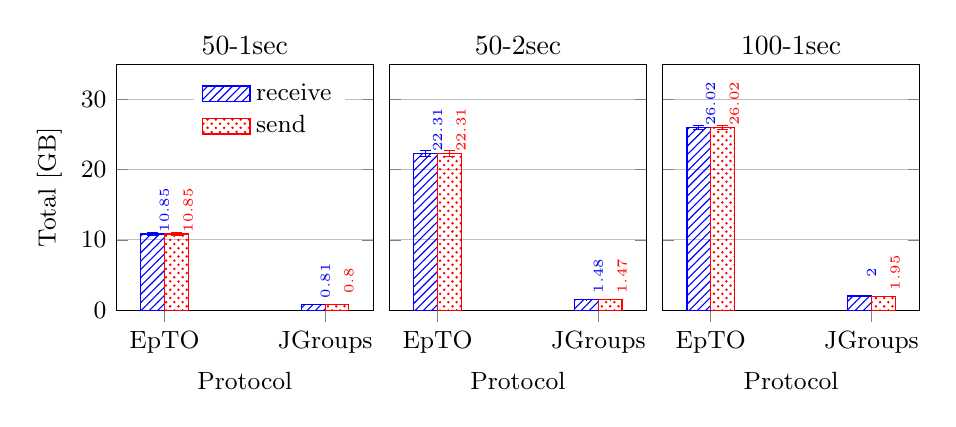
\begin{tikzpicture}
\usetikzlibrary{plotmarks}
\pgfplotsset{width=\linewidth, height=4.7cm}
\begin{groupplot}[
group style={
	group size=3 by 1,
	vertical sep=0pt,
	horizontal sep=2mm,
	xlabels at=edge bottom,
	ylabels at=edge left,
	xticklabels at=edge bottom,
	yticklabels at=edge left,
},
ymin=0,
ymax=35,
width=\linewidth / 2.5,
enlarge x limits=0.3,
ybar=0,
/pgf/bar width=3mm,
/pgfplots/area legend,
nodes near coords,
legend style={
	anchor=north west,
	at={(0.3,0.97)},
	cells={anchor=west},
	draw=none,
},
every node near coord/.append style={
	rotate=90,
	anchor=north,
	font=\tiny,
	xshift=3mm,
	yshift=0.3mm,
},
ymajorgrids,
xtick=data,
xlabel=Protocol,
ylabel={Total $\left[\si{\giga\byte}\right]$},
symbolic x coords={EpTO, JGroups},
]
\nextgroupplot
% 50-1sec
\addplot+[mark=none, pattern=north east lines,pattern color=blue, error bars/.cd,y dir=both, y explicit] coordinates {
	% Receive
	(EpTO, 10.8454953841) +- (0, 0.158556056880199)
	(JGroups, 0.8112389025) +- (0, 0.0275185471028981)
};
\addplot+[mark=none, pattern=crosshatch dots,pattern color=red, error bars/.cd,y dir=both, y explicit] coordinates {
	% Send
	(EpTO, 10.84508943053) +- (0, 0.158553532839913)
	(JGroups, 0.7979795057) +- (0, 0.0275124778152395)
};
\legend{receive, send}
\nextgroupplot
% 50-2sec
\addplot+[mark=none, pattern=north east lines,pattern color=blue, error bars/.cd,y dir=both, y explicit] coordinates {
	% Receive
	(EpTO, 22.3122950339) +- (0, 0.387040306037242)
	(JGroups, 1.481260734) +- (0, 0.0112693613185708)
};
\addplot+[mark=none, pattern=crosshatch dots,pattern color=red, error bars/.cd,y dir=both, y explicit] coordinates {
	% Send
	(EpTO, 22.3118855827) +- (0, 0.387040491969926)
	(JGroups, 1.4680794813) +- (0, 0.0112627440922006)
};
\nextgroupplot
% 100-1sec
\addplot+[mark=none, pattern=north east lines,pattern color=blue, error bars/.cd,y dir=both, y explicit] coordinates {
	% Receive
	(EpTO, 26.0194016553) +- (0, 0.2773178289900919968)
	(JGroups, 2.0044813206) +- (0, 0.0103933483299930001)
};
\addplot+[mark=none, pattern=crosshatch dots,pattern color=red, error bars/.cd,y dir=both, y explicit] coordinates {
	% Send
	(EpTO, 26.0161708501) +- (0, 0.277318407393540023)
	(JGroups, 1.9504773287) +- (0, 0.0104754176417391)
};
\end{groupplot}
%
\node[anchor=south] at (group c1r1.north) {50-1sec};
\node[anchor=south] at (group c2r1.north) {50-2sec};
\node[anchor=south] at (group c3r1.north) {100-1sec};
\end{tikzpicture}
%	\vspace{-2mm} 
%	\caption{Total bytes sent/received during an average experiment}
%	\vspace{-2mm} 
%	\label{fig:total-bandwidth}
%\end{figure}
In \autoref{table:total-bandwidth}, \epto has a worse baseline than \jgroups. This is expected as \epto sends $c*n*\log_2 n$ messages per events and \jgroups sends at least $n$ messages per event so we should have at least $c*\log_2 n$ more messages sent in \epto if \jgroups is perfect. Here we are well within this ratio.
\begin{table*}[hpt]
	\centering
	\caption{Total \si{\giga\byte} sent/received with a synthetic churn}
	\sisetup{table-format=2.2, separate-uncertainty, table-figures-uncertainty = 2, table-align-uncertainty}
	\begin{tabular}{lSSS}
		\toprule
		&& \multicolumn{2}{c}{Churn parameters} \\
		\cmidrule{3-4}
		{Protocol}&& \{1kill\}/minute & \{1kill,1add\}/minute \\
		\midrule
		\multirow{2}{*}{\epto}&{Receive}& 21.00(024) & 26.32(032)\\
							&{Sending}& 21.21(025) & 26.57(032)\\
		\midrule
		\multirow{2}{*}{\jgroups-coord}&{Receive}& 1.55(002) & 1.85(002)\\&{Sending}& 1.51(002) & 1.79(002)\\
		\midrule
		\multirow{2}{*}{\jgroups-nocoord}&{Receive}& 1.54(001) & 1.83(002)\\&{Sending}& 1.49(001) & 1.78(002)\\
		\bottomrule
	\end{tabular}
	\label{table:total-bandwidth-churn} 
\end{table*}

%\begin{figure}[h]
%	\centering
%	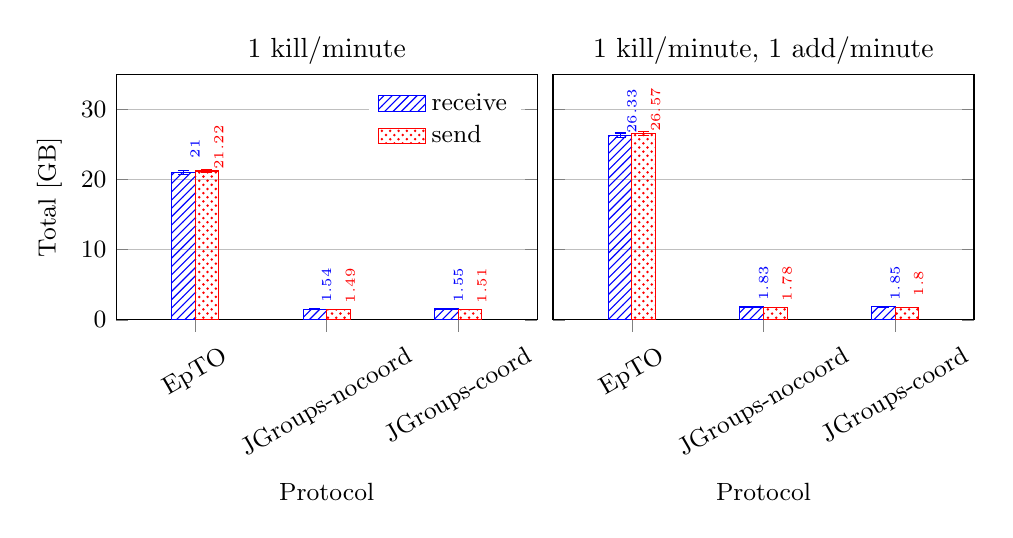
\begin{tikzpicture}
\usetikzlibrary{plotmarks}
\pgfplotsset{width=\linewidth, height=4.7cm}
\begin{groupplot}[
group style={
	group size=2 by 1,
	vertical sep=0pt,
	horizontal sep=2mm,
	xlabels at=edge bottom,
	ylabels at=edge left,
	xticklabels at=edge bottom,
	yticklabels at=edge left,
},
ymin=0,
ymax=35,
width=\linewidth / 1.75,
enlarge x limits=0.3,
ybar=0,
/pgf/bar width=3mm,
/pgfplots/area legend,
nodes near coords,
legend style={
	anchor=north west,
	at={(0.6,0.97)},
	cells={anchor=west},
	draw=none,
},
every node near coord/.append style={
	rotate=90,
	anchor=north,
	font=\tiny,
	xshift=3mm,
	yshift=0.3mm,
},
ymajorgrids,
xtick=data,
xlabel=Protocol,
xticklabel style={text height=1.5ex, rotate=30}, 
ylabel={Total $\left[\si{\giga\byte}\right]$},
symbolic x coords={EpTO, JGroups-nocoord, JGroups-coord},
]
\nextgroupplot
% 100-1sec 1kill/min
\addplot+[mark=none, pattern=north east lines,pattern color=blue, error bars/.cd,y dir=both, y explicit] coordinates {
	% Receive
	(EpTO, 21.001445292) +- (0, 0.248116313343146)
	(JGroups-nocoord, 1.5381357651) +- (0, 0.0115143286137117)
	(JGroups-coord, 1.5510862161) +- (0, 0.0181726968637206)
};
\addplot+[mark=none, pattern=crosshatch dots,pattern color=red, error bars/.cd,y dir=both, y explicit] coordinates {
	% Send
	(EpTO, 21.216776898) +- (0, 0.255744716454951)
	(JGroups-nocoord, 1.4935079775) +- (0, 0.0119366849923253)
	(JGroups-coord, 1.5064716889) +- (0, 0.0186384151121228)
};
\legend{receive, send}
\nextgroupplot
% 100-1sec 1kill, 1add/min
\addplot+[mark=none, pattern=north east lines,pattern color=blue, error bars/.cd,y dir=both, y explicit] coordinates {
	% Receive
	(EpTO, 26.325256447) +- (0, 0.320079175714576)
	(JGroups-nocoord, 1.8338254834) +- (0, 0.0187827622384514)
	(JGroups-coord, 1.8511940589) +- (0, 0.0183913437417294)
};
\addplot+[mark=none, pattern=crosshatch dots,pattern color=red, error bars/.cd,y dir=both, y explicit] coordinates {
	% Send
	(EpTO, 26.5733934455) +- (0, 0.320312180261336)
	(JGroups-nocoord, 1.7777051021) +- (0, 0.0190481557873808)
	(JGroups-coord, 1.7959073697) +- (0, 0.0189017779847593)
};
\end{groupplot}
%
\node[anchor=south] at (group c1r1.north) {1 kill/minute};
\node[anchor=south] at (group c2r1.north) {1 kill/minute, 1 add/minute};
\end{tikzpicture}
%	\vspace{-2mm} 
%	\caption{Total bytes sent/received during an average experiment with churn}
%	\vspace{-2mm} 
%	\label{fig:total-bandwidth-churn}
%\end{figure}
In \autoref{table:total-bandwidth-churn} we can see that \jgroups total bandwidth usage is smaller when there is churn. One hypothesis for this is that a JGroups replica takes a longer time to start up thus the overall benchmark has a longer time with less than 100 replicas. We also do not see a difference whether we kill the coordinator or not. This can be explained by the fact that before the detection of the faulty coordinator \jgroups is forced to a stop for time up to \SI{20}{\second}. The big spike afterwards compensates for this hole.
\subsection{Local Times}
\label{sub:local-times}
\begin{figure*}[hpt]
	\centering
	\begin{tikzpicture}
\begin{groupplot}[
group style={
	group size=3 by 1,
	vertical sep=0pt,
	horizontal sep=6mm,
	xlabels at=edge bottom,
	ylabels at=edge left,
	xticklabels at=edge bottom,
	yticklabels at=edge left,
},
every axis plot/.append style={very thick},
width=\linewidth / 3,
height=5cm,
grid=major,
grid style={dashed,gray!30},
ymax=1.05,
ymin=0,
xmin=1185,
xmax=1202.5,
xlabel={Time $\left[\si{\second}\right]$},
x tick label style={/pgf/number format/fixed},
ytick={0,0.2,0.4,0.6,0.8,1},
yticklabels={0,0.2,0.4,0.6,0.8,1},
ylabel=Percentiles,
legend columns=3,
legend cell align=left,
legend style={at={(1.6,1.4)},anchor=north, font=\small, draw=none},
cycle list name=my colors,
]
\nextgroupplot
\addplot+[const plot, mark=none] table[x=EpTO-50-1sec-x, y=EpTO-50-1sec-y, col sep=comma] {\tablelocaltime};
\addplot+[const plot, mark=none] table[x=JGroups-50-1sec-x, y=JGroups-50-1sec-y, col sep=comma] {\tablelocaltime};
\legend{EpTO, JGroups}
%
\nextgroupplot
\addplot+[const plot, mark=none] table[x=EpTO-50-2sec-x, y=EpTO-50-2sec-y, col sep=comma] {\tablelocaltime};
\addplot+[const plot, mark=none] table[x=JGroups-50-2sec-x, y=JGroups-50-2sec-y, col sep=comma] {\tablelocaltime};
%
\nextgroupplot
\addplot+[const plot, mark=none] table[x=EpTO-100-1sec-x, y=EpTO-100-1sec-y, col sep=comma] {\tablelocaltime};
\addplot+[const plot, mark=none] table[x=JGroups-100-1sec-x, y=JGroups-100-1sec-y, col sep=comma] {\tablelocaltime};
\end{groupplot}
%
\node[anchor=south] at (group c1r1.north) {$(50,50)$};
\node[anchor=south] at (group c2r1.north) {$(50,100)$};
\node[anchor=south] at (group c3r1.north) {$(100,50)$};
\end{tikzpicture}
	\vspace{-2mm} 
	\caption{Local dissemination times}
	\vspace{-2mm}
	\label{fig:local-times} 
\end{figure*}

\begin{figure}[hpt]
	\centering
	\begin{tikzpicture}
\begin{groupplot}[
group style={
group size=2 by 1,
vertical sep=0pt,
horizontal sep=6mm,
xlabels at=edge bottom,
ylabels at=edge left,
xticklabels at=edge bottom,
yticklabels at=edge left,
},
every axis plot/.append style={very thick},
height=5cm, width=\linewidth / 1.75,
grid=major,
grid style={dashed,gray!30},
ymax=1.05,
ymin=0,
xmin=1185,
xmax=1202.5,
xlabel={Time $\left[\si{\second}\right]$},
x tick label style={/pgf/number format/fixed},
ytick={0,0.2,0.4,0.6,0.8,1},
yticklabels={0,0.2,0.4,0.6,0.8,1},
ylabel=Percentiles,
legend columns=3,
legend cell align=left,
legend style={at={(1.1,1.3)},anchor=north, font=\small, draw=none},
cycle list name=my colors,
]
\nextgroupplot
\addplot+[const plot, mark=none] table[x=EpTO-suspend-x, y=EpTO-suspend-y, col sep=comma] {\tablelocaltime};
\addplot+[const plot, mark=none] table[x=JGroups-suspend-coord-x, y=JGroups-suspend-coord-y, col sep=comma] {\tablelocaltime};
\addplot+[const plot, mark=nonee] table[x=JGroups-suspend-nocoord-x, y=JGroups-suspend-nocoord-y, col sep=comma] {\tablelocaltime};
\legend{\epto, \jgroups-nocoord, \jgroups-coord}
%
\nextgroupplot
\addplot+[const plot, mark=nonek] table[x=EpTO-add-suspend-x, y=EpTO-add-suspend-y, col sep=comma] {\tablelocaltime};
\addplot+[const plot, mark=none] table[x=JGroups-add-suspend-coord-x, y=JGroups-add-suspend-coord-y, col sep=comma] {\tablelocaltime};
\addplot+[const plot, mark=none] table[x=JGroups-add-suspend-nocoord-x, y=JGroups-add-suspend-nocoord-y, col sep=comma] {\tablelocaltime};
\end{groupplot}
%
\node[anchor=south] at (group c1r1.north) {1 kill/minute};
\node[anchor=south] at (group c2r1.north) {1 \{kill,add\}/minute};
\end{tikzpicture}
	\vspace{-2mm} 
	\caption{Local dissemination times with churn}
	\vspace{-2mm} 
	\label{fig:local-times-churn} 
\end{figure}
In \autoref{fig:local-times}, \jgroups delivers all events quicker than \epto in all scenarios, even when churn is involved as is shown in \autoref{fig:local-times-churn}. However, \epto is not too far behind. The difference between \epto and \jgroups is likely to be even smaller when running them in a real WAN network due to the latency. \epto in our configuration has a $\delta$ period of \SI{100}{\milli\second} and is thus handicapped against \jgroups in a LAN environment, because it only increments the TTL of an event every \SI{100}{\milli\second}.
\subsection{Global Times}
\begin{figure*}[hpt]
	\centering
	\begin{tikzpicture}
\begin{groupplot}[
group style={
	group size=3 by 1,
	vertical sep=0pt,
	horizontal sep=6mm,
	xlabels at=edge bottom,
	ylabels at=edge left,
	xticklabels at=edge bottom,
	yticklabels at=edge left,
},
every axis plot/.append style={very thick},
width=\linewidth / 3,
height=5cm,
grid=major,
grid style={dashed,gray!30},
ymax=1.05,
ymin=0,
xmin=1185,
xmax=1202.5,
xlabel={Time $\left[\si{\second}\right]$},
x tick label style={/pgf/number format/fixed},
ytick={0,0.2,0.4,0.6,0.8,1},
yticklabels={0,0.2,0.4,0.6,0.8,1},
ylabel=Percentiles,
legend columns=3,
legend cell align=left,
legend style={at={(1.6,1.3)},anchor=north, font=\small, draw=none, fill=none},
cycle list name=my colors,
]
\nextgroupplot
\addplot+[const plot, mark=none] table[x=EpTO-50-1sec-x, y=EpTO-50-1sec-y, col sep=comma] {\tableglobaltime};
\addplot+[const plot, mark=none] table[x=JGroups-50-1sec-x, y=JGroups-50-1sec-y, col sep=comma] {\tableglobaltime};
\legend{\epto, \jgroups}
%
\nextgroupplot
\addplot+[const plot, mark=none] table[x=EpTO-50-2sec-x, y=EpTO-50-2sec-y, col sep=comma] {\tableglobaltime};
\addplot+[const plot, mark=none] table[x=JGroups-50-2sec-x, y=JGroups-50-2sec-y, col sep=comma] {\tableglobaltime};
%
\nextgroupplot
\addplot+[const plot, mark=none] table[x=EpTO-100-1sec-x, y=EpTO-100-1sec-y, col sep=comma] {\tableglobaltime};
\addplot+[const plot, mark=none] table[x=JGroups-100-1sec-x, y=JGroups-100-1sec-y, col sep=comma] {\tableglobaltime};
\end{groupplot}
%
\node[anchor=south] at (group c1r1.north) {$(50,50)$};
\node[anchor=south] at (group c2r1.north) {$(50,100)$};
\node[anchor=south] at (group c3r1.north) {$(100,50)$};
\end{tikzpicture}
	\vspace{-2mm} 
	\caption{Global dissemination times}
	\vspace{-2mm}
	\label{fig:global-times}  
\end{figure*}

\begin{figure}[hpt]
	\centering
	\begin{tikzpicture}
\begin{groupplot}[
group style={
group size=2 by 1,
vertical sep=0pt,
horizontal sep=6mm,
xlabels at=edge bottom,
ylabels at=edge left,
xticklabels at=edge bottom,
yticklabels at=edge left,
},
every axis plot/.append style={very thick},
height=5cm, width=\linewidth / 1.75,
grid=major,
grid style={dashed,gray!30},
ymax=1.05,
ymin=0,
xmin=1185,
xmax=1202.5,
xlabel={Time $\left[\si{\second}\right]$},
x tick label style={/pgf/number format/fixed},
ytick={0,0.2,0.4,0.6,0.8,1},
yticklabels={0,0.2,0.4,0.6,0.8,1},
ylabel=Percentiles,
legend columns=3,
legend cell align=left,
legend style={at={(1.1,1.3)},anchor=north, font=\small, draw=none},
cycle list name=my colors,
]
\nextgroupplot
\addplot+[const plot, mark=none] table[x=EpTO-suspend-x, y=EpTO-suspend-y, col sep=comma] {\tableglobaltime};
\addplot+[const plot, mark=none] table[x=JGroups-suspend-coord-x, y=JGroups-suspend-coord-y, col sep=comma] {\tableglobaltime};
\addplot+[const plot, mark=nonee] table[x=JGroups-suspend-nocoord-x, y=JGroups-suspend-nocoord-y, col sep=comma] {\tableglobaltime};
\legend{EpTO, JGroups-nocoord, JGroups-coord}
%
\nextgroupplot
\addplot+[const plot, mark=nonek] table[x=EpTO-add-suspend-x, y=EpTO-add-suspend-y, col sep=comma] {\tableglobaltime};
\addplot+[const plot, mark=none] table[x=JGroups-add-suspend-coord-x, y=JGroups-add-suspend-coord-y, col sep=comma] {\tableglobaltime};
\addplot+[const plot, mark=none] table[x=JGroups-add-suspend-nocoord-x, y=JGroups-add-suspend-nocoord-y, col sep=comma] {\tableglobaltime};
\end{groupplot}
%
\node[anchor=south] at (group c1r1.north) {1 kill/minute};
\node[anchor=south] at (group c2r1.north) {1 \{kill,add\}/minute};
\end{tikzpicture}
	\vspace{-2mm} 
	\caption{Global dissemination times with churn}
	\vspace{-2mm} 
	\label{fig:global-times-churn} 
\end{figure}
We computed global times as well. They are represented in \autoref{fig:global-times} and \autoref{fig:global-times-churn}. These global times are of less interest than their local counterpart as the differences in clocks between hosts can skew this measurement.

Nonetheless, here too we can see that \epto is consistently slower than \jgroups for the same reason as stated in \autoref{sub:local-times}.
\subsection{Local Dissemination stretch}
\begin{figure*}[hpt]
	\centering
	\begin{tikzpicture}
\begin{groupplot}[
group style={
	group size=3 by 1,
	vertical sep=0pt,
	horizontal sep=4mm,
	xlabels at=edge bottom,
	ylabels at=edge left,
	xticklabels at=edge bottom,
	yticklabels at=edge left,
},
every axis plot/.append style={very thick},
width=\linewidth / 2.5,
height=5cm,
grid=major,
grid style={dashed,gray!30},
ymax=1.05,
ymin=0,
xmax=3.5,
xlabel={Time $\left[\si{\second}\right]$},
x tick label style={/pgf/number format/fixed},
ytick={0,0.2,0.4,0.6,0.8,1},
yticklabels={0,0.2,0.4,0.6,0.8,1},
ylabel=Percentiles,
legend columns=3,
legend cell align=left,
legend style={at={(1.6,1.3)},anchor=north, font=\small, draw=none},
cycle list name=my colors,
]
\nextgroupplot
\addplot+[const plot, mark=none] table[x=EpTO-50-1sec-x, y=EpTO-50-1sec-y, col sep=comma] {\tablelocaldeltas};
\addplot+[const plot, mark=none] table[x=JGroups-50-1sec-x, y=JGroups-50-1sec-y, col sep=comma] {\tablelocaldeltas};
\legend{\epto, \jgroups}
%
\nextgroupplot
\addplot+[const plot, mark=none] table[x=EpTO-50-2sec-x, y=EpTO-50-2sec-y, col sep=comma] {\tablelocaldeltas};
\addplot+[const plot, mark=none] table[x=JGroups-50-2sec-x, y=JGroups-50-2sec-y, col sep=comma] {\tablelocaldeltas};
%
\nextgroupplot
\addplot+[const plot, mark=none] table[x=EpTO-100-1sec-x, y=EpTO-100-1sec-y, col sep=comma] {\tablelocaldeltas};
\addplot+[const plot, mark=none] table[x=JGroups-100-1sec-x, y=JGroups-100-1sec-y, col sep=comma] {\tablelocaldeltas};
\end{groupplot}
%
\node[anchor=south] at (group c1r1.north) {$(50,50)$};
\node[anchor=south] at (group c2r1.north) {$(50,100)$};
\node[anchor=south] at (group c3r1.north) {$(100,50)$};
\end{tikzpicture}
	\vspace{-2mm} 
	\caption{Local dissemination stretch}
	\vspace{-2mm}
	\label{fig:local-delta}  
\end{figure*}
In \autoref{fig:local-delta}, We can see the percentiles of the local dissemination stretch. The local dissemination stretch is the time measurement between the sending of an event by a peer and the delivery of this event locally.

\jgroups is usually much faster than \epto in a perfect environment. This is expected as the benchmarks involve a small number of nodes and are performed in a LAN environment with minmimal latency. The median dissemination stretch of \jgroups is around \SI{7}{\milli\second} where as the median dissemiantion stretch of \epto is around \SI{630}{\milli\second} for $(100,50)$. When increasing the number of peers, \jgroups starts to have long delivery times for some outliers.

\begin{figure}[hpt]
	\centering
	\begin{tikzpicture}
\begin{groupplot}[
group style={
	group size=2 by 1,
	vertical sep=0pt,
	horizontal sep=6mm,
	xlabels at=edge bottom,
	ylabels at=edge left,
	xticklabels at=edge bottom,
	yticklabels at=edge left,
},
every axis plot/.append style={very thick},
height=5cm, width=\linewidth / 1.75,
grid=major,
grid style={dashed,gray!30},
ymax=1.05,
ymin=0,
xmax=25,
scaled x ticks = false,
x tick label style={/pgf/number format/fixed},
xlabel={Time $\left[\si{\second}\right]$},
ytick={0,0.2,0.4,0.6,0.8,1},
yticklabels={0,0.2,0.4,0.6,0.8,1},
ylabel=Percentiles,
legend columns=3,
legend cell align=left,
legend style={at={(1.1,1.3)},anchor=north, font=\small, draw=none},
cycle list name=my colors,
]
\nextgroupplot
\addplot+[const plot, mark=none] table[x=EpTO-suspend-x, y=EpTO-suspend-y, col sep=comma] {\tablelocaldeltas};
\addplot+[const plot, mark=none] table[x=JGroups-suspend-coord-x, y=JGroups-suspend-coord-y, col sep=comma] {\tablelocaldeltas};
\addplot+[const plot, mark=nonee] table[x=JGroups-suspend-nocoord-x, y=JGroups-suspend-nocoord-y, col sep=comma] {\tablelocaldeltas};
\legend{\epto, \jgroups-coord, \jgroups-nocoord}
%
\nextgroupplot
\addplot+[const plot, mark=none] table[x=EpTO-add-suspend-x, y=EpTO-add-suspend-y, col sep=comma] {\tablelocaldeltas};
\addplot+[const plot, mark=none] table[x=JGroups-add-suspend-coord-x, y=JGroups-add-suspend-coord-y, col sep=comma] {\tablelocaldeltas};
\addplot+[const plot, mark=none] table[x=JGroups-add-suspend-nocoord-x, y=JGroups-add-suspend-nocoord-y, col sep=comma] {\tablelocaldeltas};
\end{groupplot}
%
\node[anchor=south] at (group c1r1.north) {1 kill/minute};
\node[anchor=south] at (group c2r1.north) {1 \{kill,add\}/minute};
\end{tikzpicture}
	\vspace{-2mm} 
	\caption{Local dissemination stretch with churn}
	\vspace{-2mm}
	\label{fig:local-delta-churn}   
\end{figure}
In \autoref{fig:local-delta-churn} We can see a completely different picture. When under churn, the 95th percentile of \jgroups is at \SI{31}{\milli\second} compared to \SI{14}{\milli\second} when there is no churn. The highest percentiles are at more than \SI{10}{\second}. This effect is due to the coordinator dying as we clearly see that it does not happen when we do not kill it.

The median is bigger at around \SI{9}{\milli\second}, whether we kill the coordinator or not. This shows that there are some degradation in \jgroups local dissemination stretch when under churn.

On the contrary, \epto performs very well under churn. The median degrade a bit at \SI{650}{\milli\second} with the 99th percentile being at \SI{1030}{\milli\second} compared to \SI{982}{\milli\second} when no churn is happening.
\subsection{Events sent}
\jt{Representing as a table might be better}
\begin{table}[hpt]
	\centering
	\caption{Total events sent in a stable environment}
\sisetup{table-format=6.1, separate-uncertainty, table-figures-uncertainty = 2, table-align-uncertainty}
\begin{tabular}{lSSS}
	\toprule
	& \multicolumn{3}{c}{Cluster parameters} \\
	\cmidrule{2-4}
	Protocol & {50P50E} & {50P50E} & {100P50E} \\
	\midrule
	\epto & 59993.8(33) & 119898.2(97) & 59913.0(1643) \\
	\jgroups & 59961.9(109) & 119885.7(50) & 60023.1(2871) \\
	\bottomrule
\end{tabular}
\label{table:total-events}  
\end{table}

%\begin{figure}[h]
%	\centering
%	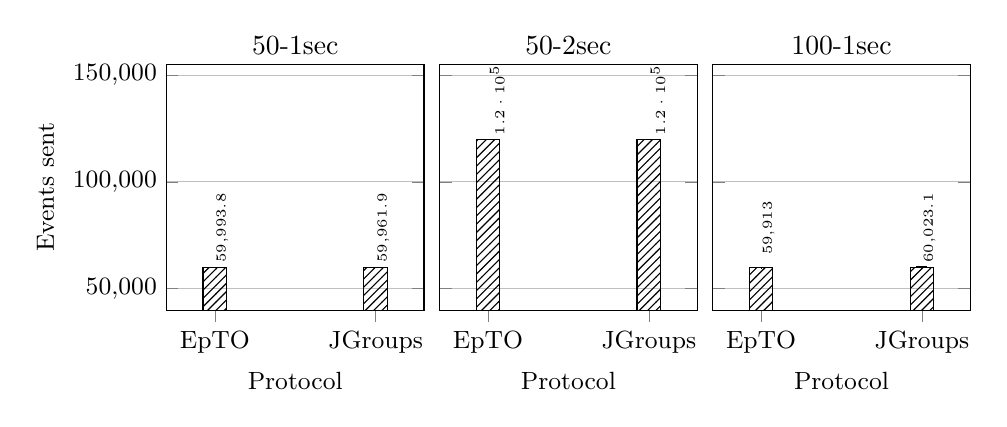
\begin{tikzpicture}
\usetikzlibrary{plotmarks}
\pgfplotsset{width=\linewidth, height=4.7cm}
\begin{groupplot}[
group style={
	group size=3 by 1,
	vertical sep=0pt,
	horizontal sep=2mm,
	xlabels at=edge bottom,
	ylabels at=edge left,
	xticklabels at=edge bottom,
	yticklabels at=edge left,
},
ymin=40000,
ymax=155000,
width=\linewidth / 2.5,
enlarge x limits=0.3,
ybar=0,
/pgf/bar width=3mm,
/pgfplots/area legend,
nodes near coords,
legend style={
	anchor=north west,
	at={(0.3,0.97)},
	cells={anchor=west},
	draw=none,
	fill=none,
},
every node near coord/.append style={
	rotate=90,
	anchor=north,
	font=\tiny,
	xshift=5mm,
	yshift=1mm,
},
ymajorgrids,
xtick=data,
xlabel=Protocol,
ylabel={Events sent},
scaled ticks=false, tick label style={/pgf/number format/fixed},
symbolic x coords={EpTO, JGroups},
]
\nextgroupplot
% 50-1sec
\addplot[mark=none, pattern=north east lines, error bars/.cd,y dir=both, y explicit] coordinates {
	% Receive
	(EpTO, 59993.8) +- (0, 3.32665998663345)
	(JGroups, 59961.9) +- (0, 10.9285558667798)
};
%
\nextgroupplot
% 50-2sec
\addplot[mark=none, pattern=north east lines, error bars/.cd,y dir=both, y explicit] coordinates {
	% Receive
	(EpTO, 119898.2) +- (0, 9.75021367287237)
	(JGroups, 119885.7) +- (0, 5.01220732035492)
};
\nextgroupplot
% 100-1sec
\addplot[mark=none, pattern=north east lines, error bars/.cd,y dir=both, y explicit] coordinates {
	% Receive
	(EpTO, 59913) +- (0, 164.332319131421)
	(JGroups, 60023.1) +- (0, 287.150928181603)
};
\end{groupplot}
%
\node[anchor=south] at (group c1r1.north) {50-1sec};
\node[anchor=south] at (group c2r1.north) {50-2sec};
\node[anchor=south] at (group c3r1.north) {100-1sec};
\end{tikzpicture}
%	\vspace{-2mm} 
%	\caption{Total events sent per experiment on average}
%	\vspace{-2mm}
%	\label{fig:total-events}   
%\end{figure}
In \autoref{table:total-events} we can see that both \epto and \jgroups deliver the same amount of events. This is expected in a perfect environment.
\begin{table}[hpt]
	\centering
	\caption{Total events sent with a synthetic churn}
\sisetup{table-format=6.1, separate-uncertainty, table-figures-uncertainty = 2, table-align-uncertainty}
\begin{tabular}{lSSS}
	\toprule
	& \multicolumn{2}{c}{Cluster parameters} \\
	\cmidrule{2-3}
	Protocol & \{1kill\}/minute & \{1kill,1add\}/minute \\
	\midrule
	\epto & 53898.5(1339) & 59798.6(1401) \\
	\jgroups-coord & 53834.7(1755) & 59507.9(2409) \\
	\jgroups-nocoord & 53830.5(2003) & 59450.5(1751) \\
	\bottomrule
\end{tabular}
    \label{table:total-events-churn}
\end{table}
%\begin{figure}[h]
%	\centering
%	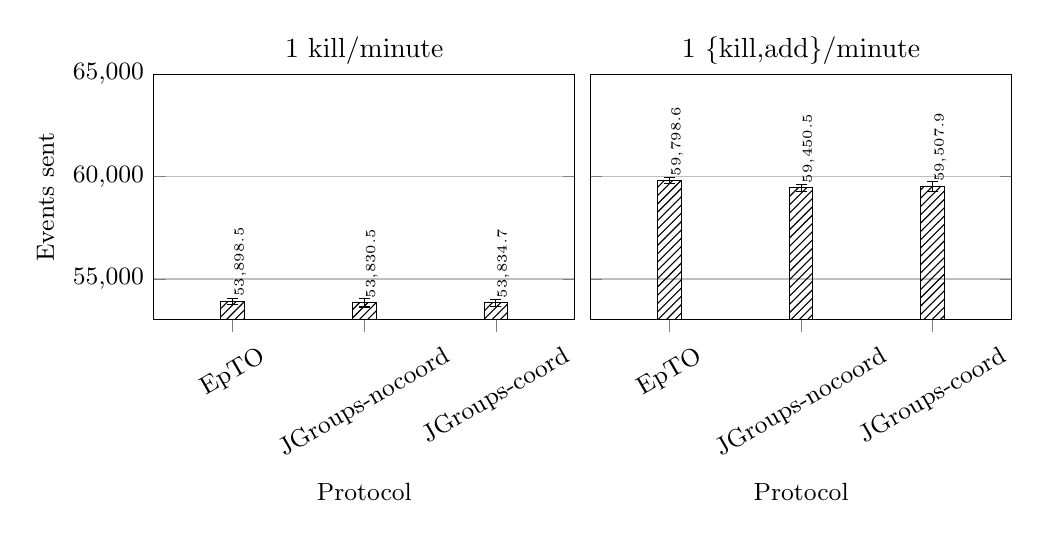
\begin{tikzpicture}
\pgfplotsset{width=\linewidth, height=4.7cm}
\begin{groupplot}[
group style={
	group size=2 by 1,
	vertical sep=0pt,
	horizontal sep=2mm,
	xlabels at=edge bottom,
	ylabels at=edge left,
	xticklabels at=edge bottom,
	yticklabels at=edge left,
},
ymin=53000,
ymax=65000,
width=\linewidth / 1.75,
enlarge x limits=0.3,
ybar=0,
/pgf/bar width=3mm,
/pgfplots/area legend,
nodes near coords,
legend style={
	anchor=north west,
	at={(0.6,0.97)},
	cells={anchor=west},
	draw=none,
	fill=none,
},
every node near coord/.append style={
	rotate=90,
	anchor=north,
	font=\tiny,
	xshift=5mm,
	yshift=1mm,
},
ymajorgrids,
xtick=data,
xlabel=Protocol,
xticklabel style={text height=1.5ex, rotate=30}, 
scaled ticks=false, tick label style={/pgf/number format/fixed},
ylabel={Events sent},
symbolic x coords={EpTO, JGroups-nocoord, JGroups-coord},
]
\nextgroupplot
% 100-1sec 1kill/min
\addplot[mark=none, pattern=north east lines, error bars/.cd,y dir=both, y explicit] coordinates {
	% Receive
	(EpTO, 53898.5) +- (0, 133.952935350029)
	(JGroups-nocoord, 53830.5) +- (0, 200.355933278752)
	(JGroups-coord, 53834.7) +- (0, 175.463861426411)
};
%
\nextgroupplot
% 100-1sec 1kill, 1add/min
\addplot[mark=none, pattern=north east lines, error bars/.cd,y dir=both, y explicit] coordinates {
	% Receive
	(EpTO, 59798.6) +- (0, 140.107260498678)
	(JGroups-nocoord, 59450.5) +- (0, 175.171820412607)
	(JGroups-coord, 59507.9) +- (0, 240.914669079693)
};
\end{groupplot}
%
\node[anchor=south] at (group c1r1.north) {1 kill/minute};
\node[anchor=south] at (group c2r1.north) {1 \{kill,add\}/minute};
\end{tikzpicture}
%	\vspace{-2mm} 
%	\caption{Total events sent per experiment during churn on average}
%	\vspace{-2mm}
%	\label{fig:total-events-churn}  
%\end{figure}

In \autoref{table:total-events-churn} When only killing nodes, \epto and \jgroups again deliver the same amount of events. When killing and adding nodes, JGroups seems to deliver a smaller amount of nodes, however it does not look significant \jt{I didn't run any statistical analysis}
\subsection{Real Trace}
\subsubsection{Bandwidth}
\begin{figure}[hpt]
	\centering
	\begin{tikzpicture}
\usetikzlibrary{plotmarks}
\pgfplotsset{
	height=4cm,
	width=\linewidth,
	every axis plot post/.append style={
		solid,
		very thin,
		mark=none
	},
	/pgfplots/area cycle list/.style={/pgfplots/cycle list={%
			{black,fill=black,mark=none},%
			{black,fill=white!25!black,mark=none},%
			{black,fill=white!50!black,mark=none},%
			{black,fill=white!75!black,mark=none},%
			{black,fill=white,mark=none},%
		}
	},
}
\begin{groupplot}[
ymajorgrids,
group style={
	group size=1 by 4,
	vertical sep=6mm,
	horizontal sep=0mm,
	xlabels at=edge bottom,
	xticklabels at=edge bottom,
	ylabels at=edge left,
},
stack plots=y,area style, enlarge x limits=false, 
ymin=0,
xmin=0,
xmax=61,
ylabel={Bandwidth $\left[\SI{}{\mbps}\right]$},
xlabel={Time $\left[\si{\minute}\right]$},
legend columns=5,
legend cell align=left,
legend style={at={(0.2,2)},anchor=north, font=\small, draw=none},]
\nextgroupplot[height=2.2cm, 
ylabel={Nodes}, 
ymin=80,ymax=120,
ytick={80,120}, 
yticklabels={80,...,120},
xmajorgrids,
yminorgrids,
tick label style={font=\footnotesize},
label style={font=\tiny}]
\addplot[const plot, color=blue, mark=none] table [x=minute, y=size, col sep=comma] {csv-data/real-trace.csv};
\nextgroupplot[ymax=4,ytick={0,1,2,3,4},
yticklabels={0,1,2,3,4}]
\addplot table[x=time,y=EpTO-real-trace-0.000000, col sep=comma]{\tableaverage} \closedcycle;
\addplot table[x=time,y=EpTO-real-trace-0.250000, col sep=comma]{\tableaverage} \closedcycle;
\addplot table[x=time,y=EpTO-real-trace-0.500000, col sep=comma]{\tableaverage} \closedcycle;
\addplot table[x=time,y=EpTO-real-trace-0.750000, col sep=comma]{\tableaverage} \closedcycle;
\addplot table[x=time,y=EpTO-real-trace-1.000000, col sep=comma]{\tableaverage} \closedcycle;
\legend{0, 0.25, 0.5, 0.75, 1}
%
\nextgroupplot%[ymax=4,ytick={0,1,2,3,4},]
\addplot table[x=time,y=JGroups-coord-0.000000, col sep=comma]{\tableaverage} \closedcycle;
\addplot table[x=time,y=JGroups-coord-0.250000, col sep=comma]{\tableaverage} \closedcycle;
\addplot table[x=time,y=JGroups-coord-0.500000, col sep=comma]{\tableaverage} \closedcycle;
\addplot table[x=time,y=JGroups-coord-0.750000, col sep=comma]{\tableaverage} \closedcycle;
\addplot table[x=time,y=JGroups-coord-1.000000, col sep=comma]{\tableaverage} \closedcycle;
%
\nextgroupplot[ymax=4,ytick={0,1,2,3,4}]
\addplot table[x=time, y=JGroups-nocoord-0.000000, col sep=comma]{\tableaverage} \closedcycle;
\addplot table[x=time,y=JGroups-nocoord-0.250000, col sep=comma]{\tableaverage} \closedcycle;
\addplot table[x=time,y=JGroups-nocoord-0.500000, col sep=comma]{\tableaverage} \closedcycle;
\addplot table[x=time,y=JGroups-nocoord-0.750000, col sep=comma]{\tableaverage} \closedcycle;
\addplot table[x=time,y=JGroups-nocoord-1.000000, col sep=comma]{\tableaverage} \closedcycle;
\end{groupplot}
%
\node[anchor=south, rotate=-90] at (group c1r2.east) {EpTO};
\node[anchor=south, rotate=-90] at (group c1r3.east) {JGroups coord};
\node[anchor=south, rotate=-90] at (group c1r4.east) {JGroups nocoord};
\end{tikzpicture}
	\vspace{-2mm} 
	\caption{Throughput percentiles of a node during an experiment with churn}
	\vspace{-2mm} 
	\label{fig:bandwidth-real-churn}
\end{figure}
\subsubsection{Total Bytes sent/received}
\begin{table}[hpt]
	\centering
	\caption{Total \si{\giga\byte} sent/received}
	\sisetup{table-format=2.2, separate-uncertainty, table-figures-uncertainty = 2, table-align-uncertainty}
	\begin{tabular}{lSS}
		\toprule
		&& \multicolumn{1}{c}{Churn parameters} \\
		\cmidrule{3-3}
		{Protocol}&& {Real Trace} \\
		\midrule
		\multirow{2}{*}{\epto}&{Receive}& 81.41(108)\\
		&{Sending}& 82.67(108)\\
		\midrule
		\multirow{2}{*}{\jgroups-coord}&{Receive}& 5.61(008)\\
		&{Sending}& 5.45(008)\\
		\midrule
		\multirow{2}{*}{\jgroups-nocoord}&{Receive}& 5.63(005)\\
		&{Sending}& 5.48(005)\\
		\bottomrule
	\end{tabular}
	\label{table:total-bandwidth-real-churn} 
\end{table}
%\begin{figure}[h]
%	\centering
%	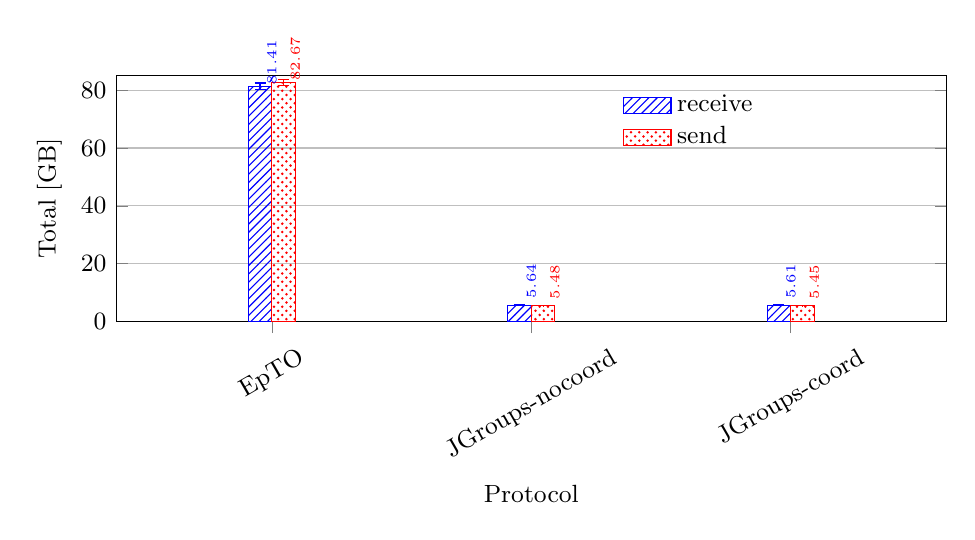
\begin{tikzpicture}
\usetikzlibrary{plotmarks}
\pgfplotsset{width=\linewidth, height=4.7cm}
\begin{axis}[
ymin=0,
ymax=85,
enlarge x limits=0.3,
ybar=0,
/pgf/bar width=3mm,
/pgfplots/area legend,
nodes near coords,
legend style={
	anchor=north west,
	at={(0.6,0.97)},
	cells={anchor=west},
	draw=none,
	fill=none,
},
every node near coord/.append style={
	rotate=90,
	anchor=north,
	font=\tiny,
	xshift=3mm,
	yshift=0.3mm,
},
ymajorgrids,
xtick=data,
xlabel=Protocol,
xticklabel style={text height=1.5ex, rotate=30}, 
ylabel={Total $\left[\si{\giga\byte}\right]$},
symbolic x coords={EpTO, JGroups-nocoord, JGroups-coord},
]
% 100-1sec 1kill/min
\addplot+[mark=none, pattern=north east lines,pattern color=blue, error bars/.cd,y dir=both, y explicit] coordinates {
	% Receive
	(EpTO, 81.4132665062) +- (0, 1.0822819001435)
	(JGroups-nocoord, 5.6382174422) +- (0, 0.058029870294168)
	(JGroups-coord, 5.6118450728) +- (0, 0.089291024953546)
};
\addplot+[mark=none, pattern=crosshatch dots,pattern color=red, error bars/.cd,y dir=both, y explicit] coordinates {
	% Send
	(EpTO, 82.6741897528) +- (0, 1.08368411575119)
	(JGroups-nocoord, 5.4807749566) +- (0, 0.056977818312573)
	(JGroups-coord, 5.4548362802) +- (0, 0.086273738554255)
};
\legend{receive, send}
\end{axis}
\end{tikzpicture}
%	\vspace{-2mm} 
%	\caption{Total bytes sent/received during an average experiment with churn}
%	\vspace{-2mm} 
%	\label{fig:total-bandwidth-real-churn}
%\end{figure}

\subsubsection{Local Times}
\begin{figure}[hpt]
	\centering
	\begin{tikzpicture}
\begin{axis}[
every axis plot/.append style={very thick},
height=5cm,
grid=major,
grid style={dashed,gray!30},
ymax=1.05,
ymin=0,
xlabel={Time $\left[\si{\second}\right]$},
x tick label style={/pgf/number format/fixed},
ytick={0,0.2,0.4,0.6,0.8,1},
yticklabels={0,0.2,0.4,0.6,0.8,1},
xmin=3649,
xmax=3663,
xtick={3650,3655,3660},
xticklabels={3650,3655,3660},
ylabel=Percentiles,
legend columns=3,
legend cell align=left,
legend style={at={(0.5,1.2)},anchor=north, font=\small, draw=none},
cycle list name=my colors,
]
\addplot+[const plot, mark=none] table[x=EpTO-real-trace-x, y=EpTO-real-trace-y, col sep=comma] {\tablelocaltime};
\addplot+[const plot, mark=none] table[x=JGroups-coord-x, y=JGroups-coord-y, col sep=comma] {\tablelocaltime};
\addplot+[const plot, mark=nonee] table[x=JGroups-nocoord-x, y=JGroups-nocoord-y, col sep=comma] {\tablelocaltime};
\legend{\epto, \jgroups-nocoord, \jgroups-coord}
\end{axis}
\end{tikzpicture}
	\vspace{-2mm} 
	\caption{Local dissemination times}
	\vspace{-2mm}
	\label{fig:local-times-real-churn} 
\end{figure}

\subsubsection{Global Times}

\begin{figure}[hpt]
	\centering
	\begin{tikzpicture}
\begin{axis}[
every axis plot/.append style={very thick},
height=5cm,
grid=major,
grid style={dashed,gray!30},
ymax=1.05,
ymin=0,
xlabel={Time $\left[\si{\second}\right]$},
x tick label style={/pgf/number format/fixed},
ytick={0,0.2,0.4,0.6,0.8,1},
yticklabels={0,0.2,0.4,0.6,0.8,1},
xmin=3649,
xmax=3663,
xtick={3650,3655,3660},
xticklabels={3650,3655,3660},
ylabel=Percentiles,
legend columns=3,
legend cell align=left,
legend style={at={(0.5,1.2)},anchor=north, font=\small, draw=none},
cycle list name=my colors,
]
\addplot+[const plot, mark=none] table[x=EpTO-real-trace-x, y=EpTO-real-trace-y, col sep=comma] {\tableglobaltime};
\addplot+[const plot, mark=none] table[x=JGroups-coord-x, y=JGroups-coord-y, col sep=comma] {\tableglobaltime};
\addplot+[const plot, mark=nonee] table[x=JGroups-nocoord-x, y=JGroups-nocoord-y, col sep=comma] {\tableglobaltime};
\legend{\epto, \jgroups-nocoord, \jgroups-coord}
\end{axis}
\end{tikzpicture}
	\vspace{-2mm} 
	\caption{Global dissemination times with churn}
	\vspace{-2mm} 
	\label{fig:global-times-real-churn} 
\end{figure}
\subsubsection{Local Dissemination stretch}

\begin{figure}[hpt]
	\centering
	\begin{tikzpicture}
\begin{axis}[
every axis plot/.append style={very thick},
height=5cm,
grid=major,
grid style={dashed,gray!30},
ymax=1.05,
ymin=0,
scaled x ticks = false,
x tick label style={/pgf/number format/fixed},
xlabel={Time $\left[\si{\second}\right]$},
ytick={0,0.2,0.4,0.6,0.8,1},
yticklabels={0,0.2,0.4,0.6,0.8,1},
ylabel=Percentiles,
legend columns=3,
legend cell align=left,
legend style={at={(0.5,1.2)},anchor=north, font=\small, draw=none},
cycle list name=my colors,
]
\addplot+[const plot, mark=none] table[x=EpTO-real-trace-x, y=EpTO-real-trace-y, col sep=comma] {\tablelocaldeltas};
\addplot+[const plot, mark=none] table[x=JGroups-coord-x, y=JGroups-coord-y, col sep=comma] {\tablelocaldeltas};
\addplot+[const plot, mark=nonee] table[x=JGroups-nocoord-x, y=JGroups-nocoord-y, col sep=comma] {\tablelocaldeltas};
\legend{EpTO, JGroups-coord, JGroups-nocoord}
\end{axis}
\end{tikzpicture}
	\vspace{-2mm} 
	\caption{Local dissemination stretch with churn}
	\vspace{-2mm}
	\label{fig:local-delta-real-churn}   
\end{figure}
\subsubsection{Events sent}
\begin{table}[hpt]
	\centering
	\caption{Total events sent during a real trace}
\sisetup{table-format=6.1, separate-uncertainty, table-figures-uncertainty = 6, table-align-uncertainty}
\begin{tabular}{lS}
	\toprule
	Protocol &\\
	\midrule
	\epto & 165844.2(2102)\\
	\jgroups-coord & 166183.0(13681)\\
	\jgroups-nocoord & 166585.8(8249)\\
	\bottomrule
\end{tabular}
    \label{table:total-sent-real-churn}
\end{table}
%\begin{figure}[h]
%	\centering
%	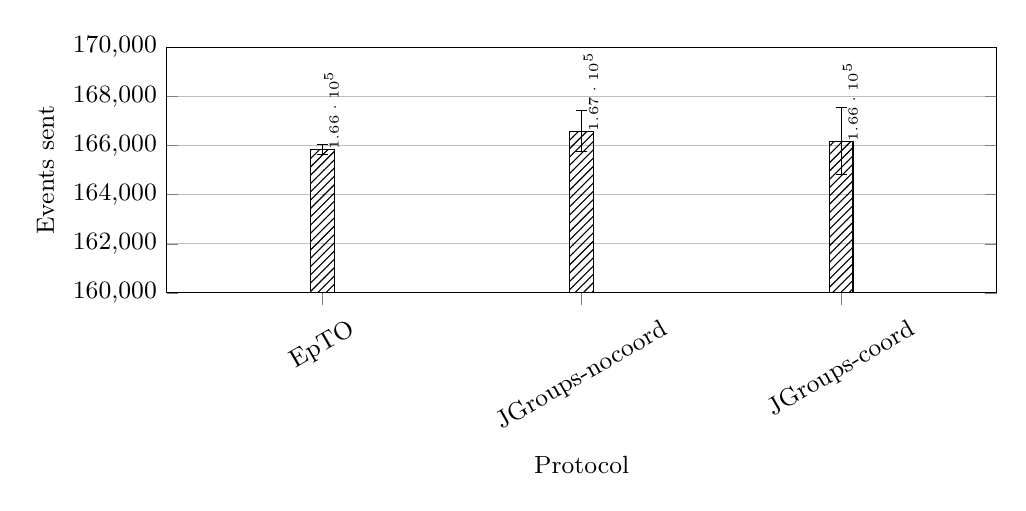
\begin{tikzpicture}
\pgfplotsset{width=\linewidth, height=4.7cm}
\begin{axis}[
ymin=160000,
ymax=170000,
enlarge x limits=0.3,
ybar=0,
/pgf/bar width=3mm,
/pgfplots/area legend,
nodes near coords,
legend style={
	anchor=north west,
	at={(0.6,0.97)},
	cells={anchor=west},
	draw=none,
	fill=none
},
every node near coord/.append style={
	rotate=90,
	anchor=north,
	font=\tiny,
	xshift=5mm,
	yshift=1mm,
},
ymajorgrids,
xtick=data,
xlabel=Protocol,
xticklabel style={text height=1.5ex, rotate=30}, 
scaled ticks=false, tick label style={/pgf/number format/fixed},
ylabel={Events sent},
symbolic x coords={EpTO, JGroups-nocoord, JGroups-coord},
]
% 100-1sec real trace
\addplot[mark=none, pattern=north east lines, error bars/.cd,y dir=both, y explicit] coordinates {
	% Events sent
	(EpTO, 165844.2) +- (0, 210.222976860287)
	(JGroups-nocoord, 166585.8) +- (0, 824.998303028558)
	(JGroups-coord, 166183) +- (0, 1368.95507596122)
};
\end{axis}
\end{tikzpicture}
%	\vspace{-2mm} 
%	\caption{Total events sent per experiment during churn on average}
%	\vspace{-2mm}
%	\label{fig:total-events-real-churn}  
%\end{figure}

\section{Future Work}
\label{sec:future-work}
\jt{Speak about running test on a bigger infrastructure, because the small ammount of nodes does not let us see the full potential of \epto. Then speak about the ongoing work of Push-Pull}
\section{Conclusion}
\label{sec:conclusion}
\jt{Do later}
\printbibliography
\end{document}
